\documentclass[10pt,a4paper]{article}
\usepackage{fontspec}\usepackage[french]{babel}
\usepackage{amsmath,amssymb,geometry,graphicx,booktabs,hyperref}
\geometry{margin=2cm}\hypersetup{colorlinks=true,urlcolor=blue,hypertexnames=false}
\setlength{\emergencystretch}{3em}
\title{SLFE : supports mobiles\\et transfert de mémoire}
\author{Recherche GPU sur le fork keckj/rodin}\date{17/11/2026 à 00:34}
\begin{document}\maketitle
Résultats disponibles le 17/11/2026 à 00:34 (Europe/Paris). Calculs en double précision sur une RTX 5090. Les figures représentent les solutions calculées, avec une référence indépendante par caractéristiques.

\section{Résultat et portée}
Un support auxiliaire mobile résout le défaut observé lorsque la bosse quitte la zone fine d'une grille fixe. Le couplage FE avec mémoire accepte désormais un changement de support contractant, et un raffinement exactement emboîté sans perte d'énergie. Les formules s'exécutent sans racine ni inversion de matrice. Ces propriétés sont démontrées dans restart\_theory.pdf et vérifiées sur GPU; elles n'établissent ni une nouveauté bibliographique, ni une convergence générale vers l'EDP.

Deux méthodes sont distinguées : le couplage avec mémoire maintient le champ FE à chaque changement; la référence d'advection pure transporte uniquement le champ DG auxiliaire entre une projection FE initiale et une projection FE finale. Cette seconde méthode est la plus rapide ici, mais elle n'offre pas les opérations physiques FE intermédiaires du couplage.

\begin{figure}[htbp]\centering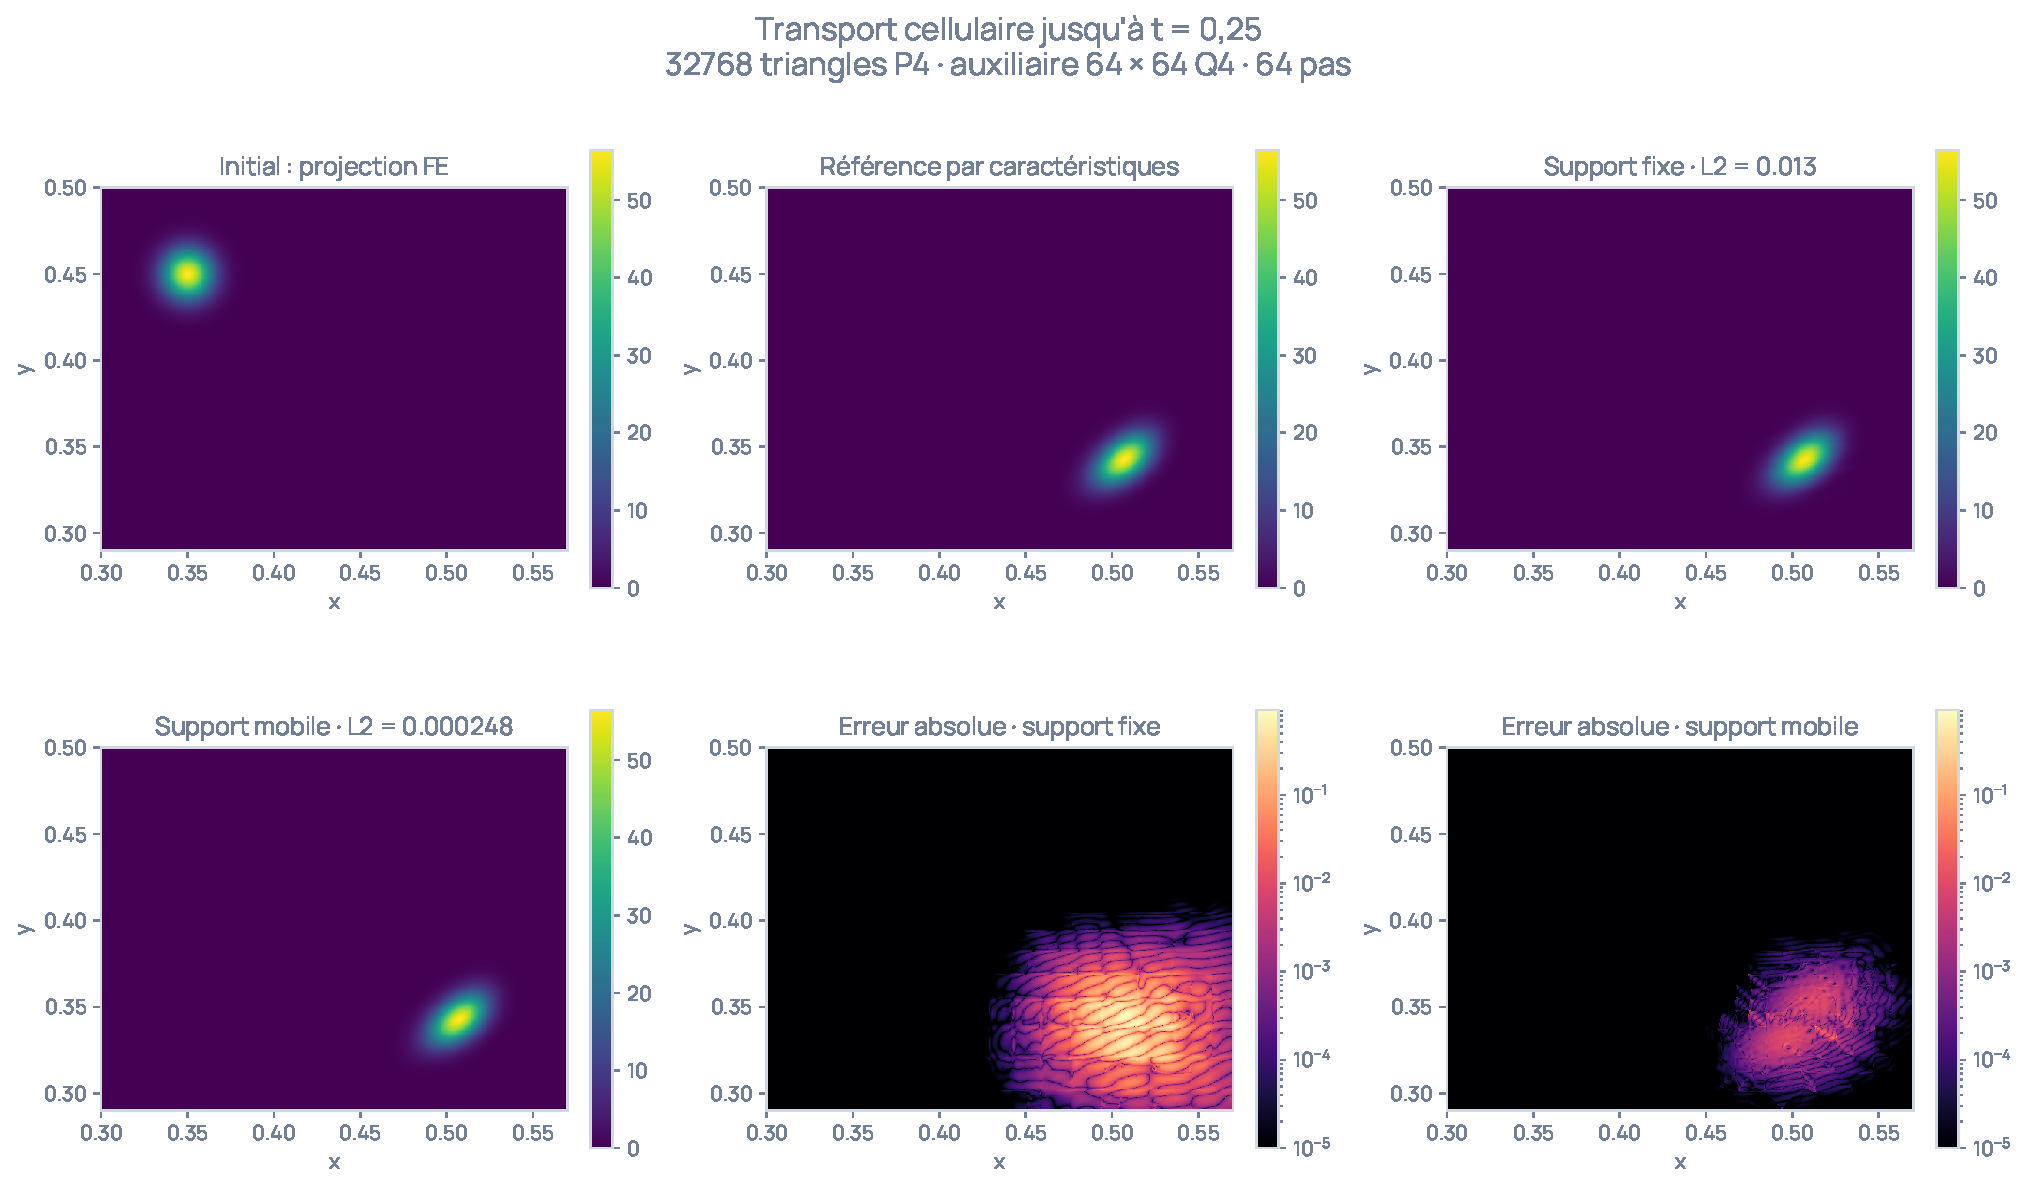
\includegraphics[width=.95\linewidth]{night-fields.pdf}\caption{Même domaine et mêmes échelles de couleur. Champ initial, référence, supports fixe et mobile, puis erreurs absolues. Le tracé est un échantillonnage FE; l'erreur L2 est intégrée séparément sur les triangles.}\end{figure}
\section{Problème et protocole}
Le domaine est le tore unité. Une vitesse cellulaire incompressible prescrite transporte jusqu'à t=0,25 une bosse de largeur 0,01, initialement centrée en (0,35; 0,45), de norme L2 proche de 1. L'espace FE principal possède 32768 triangles DG P4, soit 491520 coefficients par champ; la graduation fixe vaut 0,95. Le support principal auxiliaire comporte 64\(\times\)64 cellules Q4, soit 102400 valeurs par champ. Deux supports orientés supplémentaires servent aux cisaillements diagonaux. Les méthodes n'ont donc pas le même nombre d'inconnues.

Le centre circulaire de l'énergie est calculé à partir de la solution, tous les quatre pas. Le support se déplace lorsque ce centre s'éloigne de plus de 0,03. Ce critère convient à une structure localisée; il n'est pas un estimateur d'erreur et ne traite pas plusieurs structures éloignées. La référence intègre les caractéristiques sur GPU par 512 pas RK4; les erreurs sont intégrées avec quadrature de degré 20 et subdivision indépendante. Les extrema sont échantillonnés.

\begin{figure}[htbp]\centering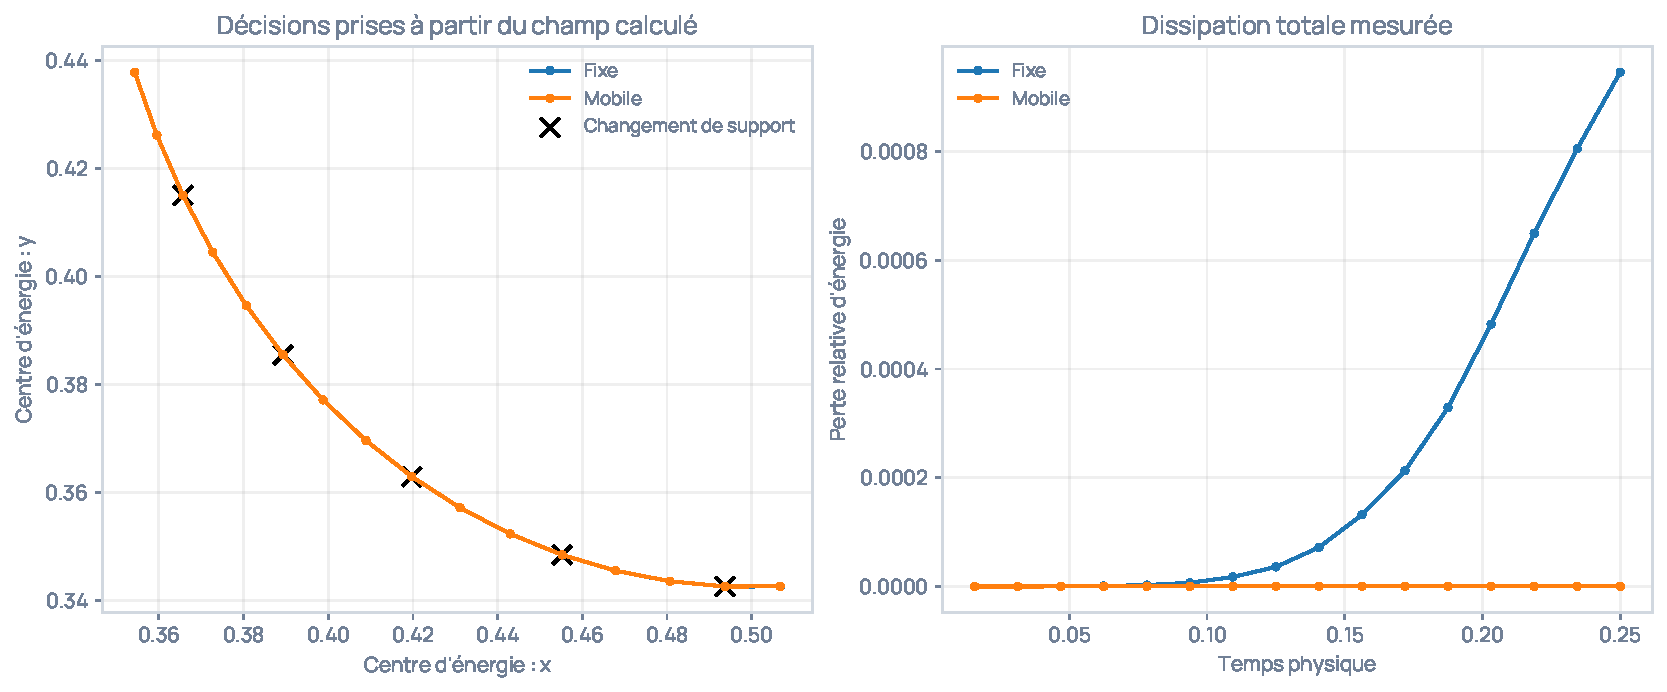
\includegraphics[width=.95\linewidth]{night-trajectory.pdf}\caption{Trajectoire du centre d'énergie et dissipation observée. Les croix indiquent les changements décidés à partir du champ numérique.}\end{figure}
\section{Précision du support mobile}
\begin{figure}[htbp]\centering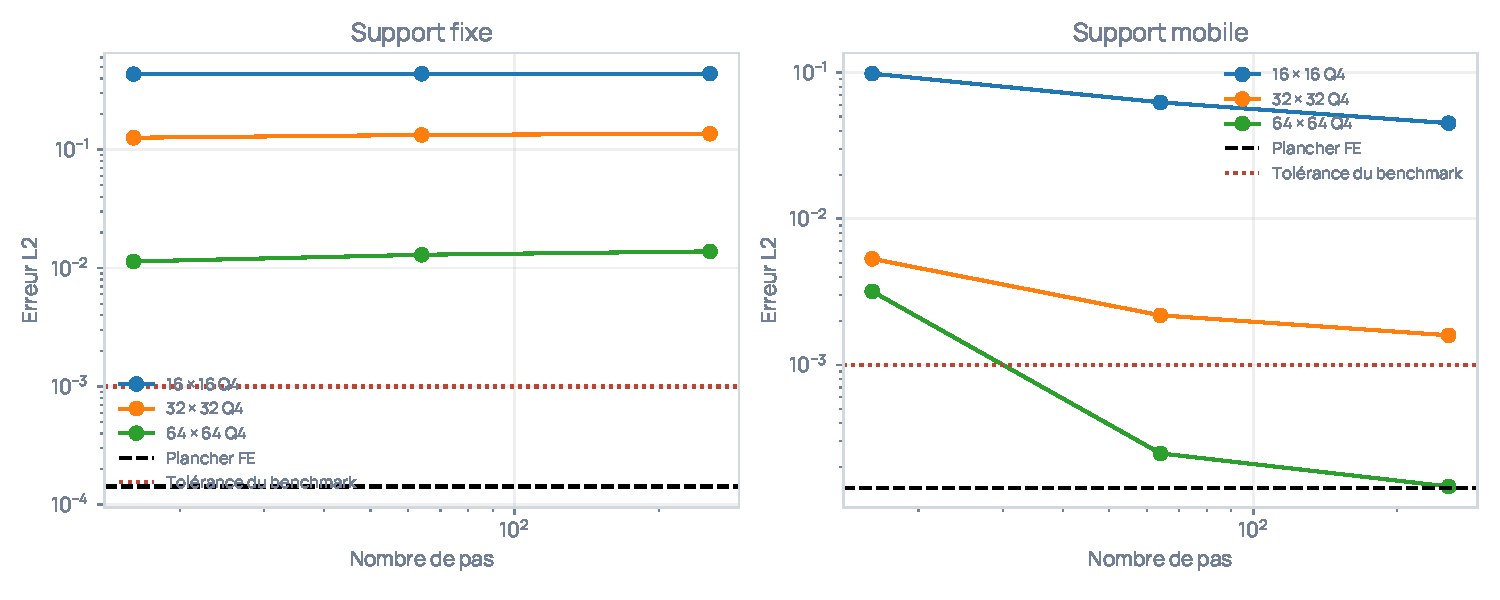
\includegraphics[width=.95\linewidth]{night-convergence.pdf}\caption{À support fixe, réduire le pas ne corrige pas le manque de résolution le long de la trajectoire. Aucune pente temporelle universelle n'est revendiquée pour cette composition avec projections.}\end{figure}
\section{Coût complet à précision imposée}
Trois répétitions alternent DG eulérien et support mobile pour 1, 4 et 16 champs distincts et proches spatialement (graine 752). Chaque champ doit satisfaire L2 \(\leq\) 0,001. Le coût inclut construction des opérateurs, détection initiale du centre, évolution, adaptations et transfert final. Le maillage FE et la projection initiale communs, ainsi que les diagnostics de référence, sont exclus des deux côtés. La compilation CUDA utilise le cache; ce ne sont pas des mesures de premier lancement sans cache.

\begin{figure}[htbp]\centering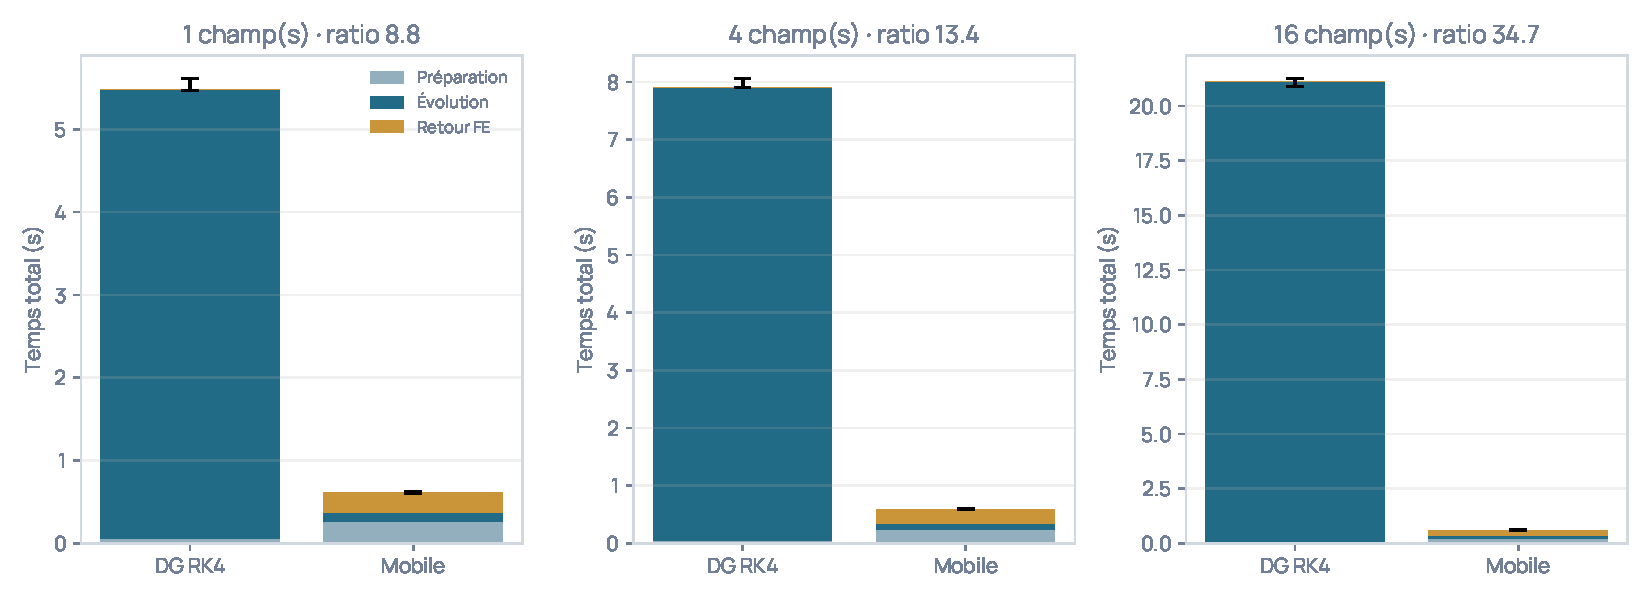
\includegraphics[width=.95\linewidth]{night-cost.pdf}\caption{Médiane et étendue des trois répétitions. Gain mesuré contre un DG amont RK4 à pas global sur ce maillage fortement gradué. Un DG à pas locaux et un solveur SL-DG GPU externe ne sont pas encore comparés.}\end{figure}
\begin{center}\small\begin{tabular}{llllll}\toprule
Champs & DG (s) & Mobile (s) & Ratio & L2 DG max & L2 mobile max\\\midrule
1 & 5.475 & 0.6195 & 8.838 & 0.0002865 & 0.0002478\\
4 & 7.908 & 0.5916 & 13.37 & 0.0008215 & 0.0004813\\
16 & 21.12 & 0.6091 & 34.67 & 0.000877 & 0.0004549\\
\bottomrule\end{tabular}\end{center}
Le pas DG retenu passe un contrôle de croissance sur champs aléatoires et la tolérance finale. Le réglage plus agressif (échelle 12) est rejeté : le contrôle aléatoire révèle une croissance d'énergie supérieure au seuil. Ce contrôle fini n'est pas un certificat spectral de stabilité. La variante mobile à 16 pas échoue à la tolérance; le benchmark utilise 64 pas.

\section{Mémoire : changement d'espace sans changer le champ FE}
L'état est représenté par trois tableaux (v,w,a), avec v=R*w+(I-R*R)a. Son énergie est ||w||\(^{2}\)+||a||\(^{2}\)-||Ra||\(^{2}\). La remise à zéro conserve v mais perd toute la mémoire invisible dans ce champ. Le transfert contractant conserve une partie de cette mémoire. En cas de raffinement exactement emboîté, l'injection corrige w par les nouveaux modes de a et préserve toute l'énergie augmentée.

\begin{center}\small\begin{tabular}{llll}\toprule
FE n & Remise à zéro L2 & Mémoire L2 & Plancher FE\\\midrule
64 & 0.006198 & 0.003851 & 0.003729\\
128 & 0.0001984 & 0.0001602 & 0.0001427\\
\bottomrule\end{tabular}\end{center}
\begin{figure}[htbp]\centering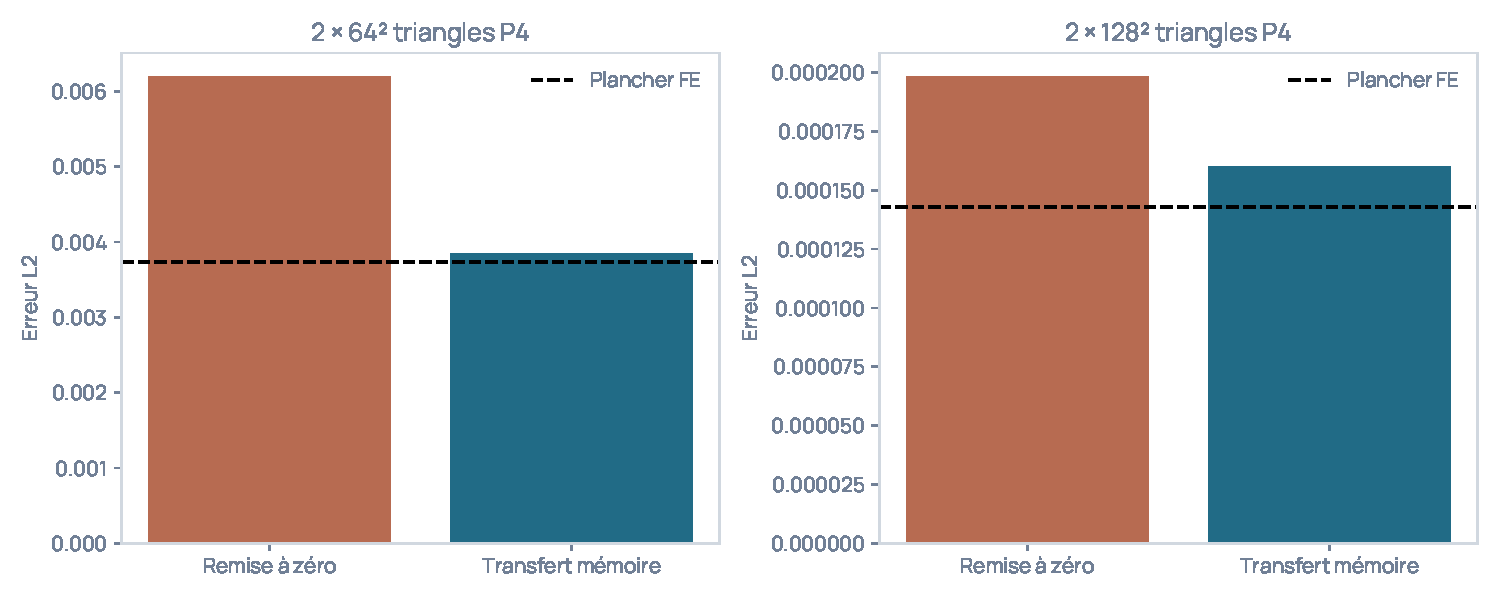
\includegraphics[width=.95\linewidth]{night-memory.pdf}\caption{Six changements de support, 128 pas et auxiliaire 64\(\times\)64 Q4. Le transfert de mémoire améliore ici l'erreur finale; la contraction seule ne garantit pas cette amélioration pour toute EDP.}\end{figure}
Une projection itérative supplémentaire utilise le recouvrement des deux espaces dans le même L2. Son filtre spectral contractant conserve davantage de mémoire lorsque le nombre d'itérations augmente. Cela ne garantit pas une diminution de l'erreur de transport. Les résultats ci-dessous sont rapportés séparément.

\begin{center}\small\begin{tabular}{llll}\toprule
FE n & Itérations & L2 & Coût total (s)\\\midrule
64 & 1 & 0.003825 & 0.9891\\
64 & 2 & 0.003782 & 0.9307\\
64 & 4 & 0.003753 & 0.9062\\
64 & 8 & 0.003739 & 0.9432\\
64 & 16 & 0.003733 & 0.9106\\
128 & 1 & 0.0001574 & 1.923\\
128 & 2 & 0.000156 & 1.87\\
128 & 4 & 0.0001551 & 1.911\\
128 & 8 & 0.0001548 & 1.931\\
128 & 16 & 0.0001547 & 1.9\\
\bottomrule\end{tabular}\end{center}
\begin{figure}[htbp]\centering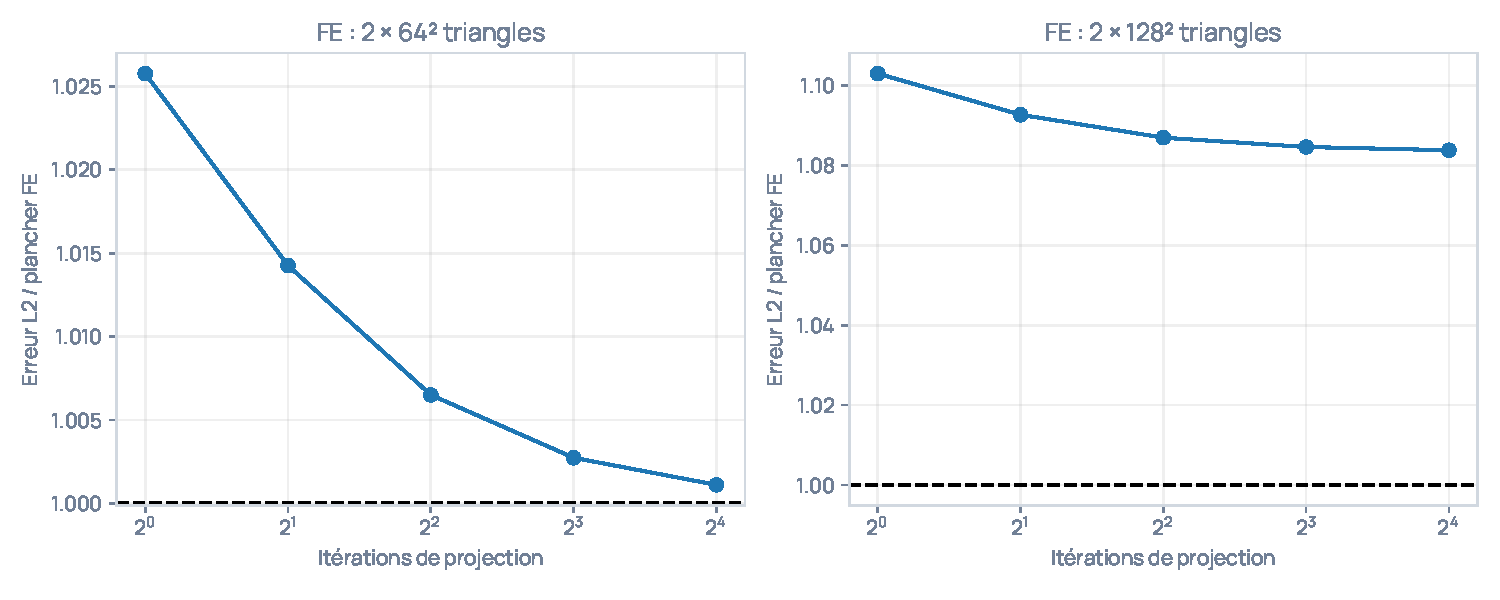
\includegraphics[width=.95\linewidth]{night-projected.pdf}\caption{Conserver davantage de mémoire rapproche ici le résultat du plancher spatial. La projection itérative utilise le recouvrement physique des espaces, condition plus forte qu'un simple remap contractant.}\end{figure}
\section{Couplage avec une réaction FE spatiale}
Une réaction de taux 1+0,5 sin(2\(\pi\)x) est appliquée par l'exponentielle exacte de son générateur Galerkin local, en deux demi-pas autour de chaque advection. Chaque mise à jour FE est réinjectée dans la mémoire. La référence indépendante intègre simultanément la trajectoire et l'exposant de réaction. L'énergie doit décroître; la masse n'est plus conservée par cette EDP.

\begin{figure}[htbp]\centering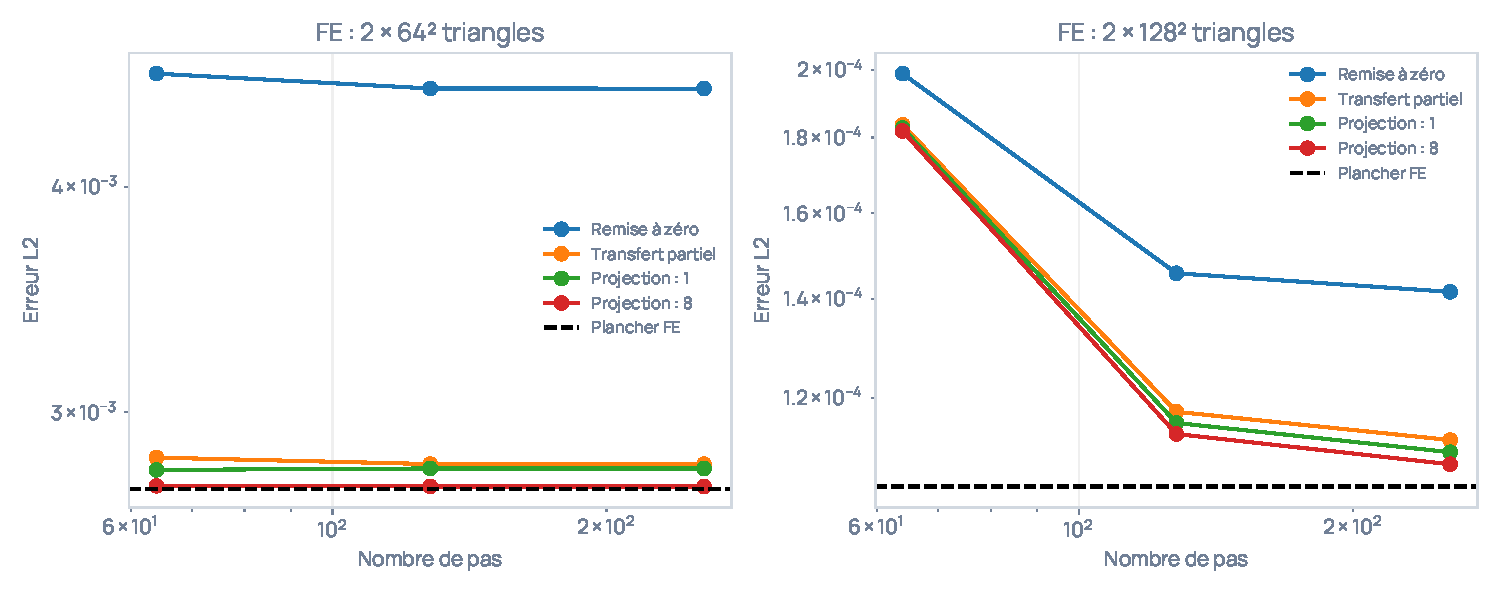
\includegraphics[width=.95\linewidth]{night-physics.pdf}\caption{Transport et réaction calculés sur GPU. L'amélioration due à la projection de mémoire persiste dans ce couplage linéaire; cela ne valide pas encore une physique non linéaire ou un transport à vitesse FE générale.}\end{figure}
\section{Accélération de la projection de mémoire}
Le carré d'un résidu de Chebyshev fournit un filtre compris entre zéro et un sur tout le spectre admissible, même sous l'échelle de ciblage choisie. Il conserve donc la contraction et l'observation FE à chaque troncature. Les techniques polynomiales sont classiques; l'intérêt mesuré ici concerne leur insertion dans le transfert de mémoire. L'échelle 0,1 fonctionne mieux que 0,01 sur ce cas; aucune supériorité universelle du réglage n'est établie.

\begin{figure}[htbp]\centering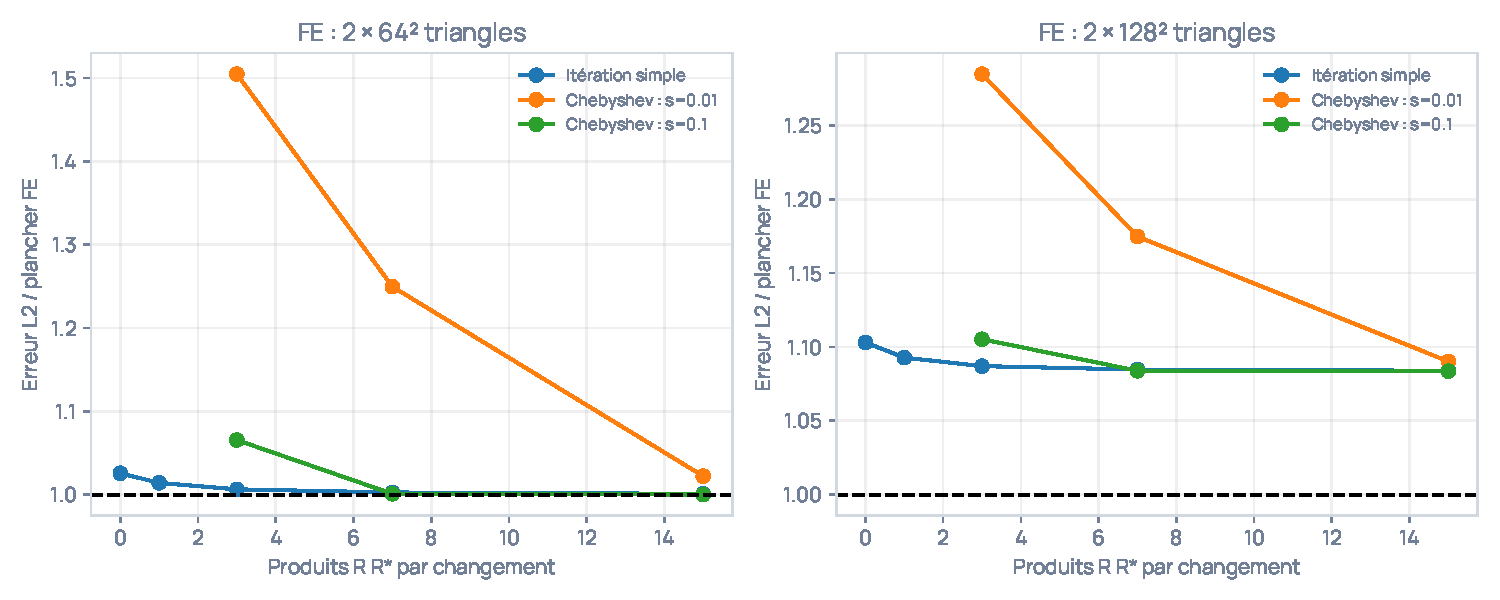
\includegraphics[width=.95\linewidth]{night-chebyshev.pdf}\caption{Coût algébrique du filtre, hors transferts communs de préparation. Sept produits avec le filtre ciblé à 0,1 atteignent ici la précision de quinze produits avec l'itération simple. Les reconstructions géométriques restent dominantes dans le temps total.}\end{figure}
Les trois transferts subissent chacun 2000 changements entre trois supports de graduations 0, 0,95 et 0,9999, entrelacés avec cisaillements et rotations locales de modes FE. Ces rotations sont un test algébrique isométrique, pas une réaction physique. Quatre champs aléatoires sont suivis; le champ FE est inchangé bit à bit au transfert.

\begin{center}\small\begin{tabular}{llll}\toprule
Transfert & Changements & Défaut FE relatif max & Défaut masse max\\\midrule
partial & 2000 & 6.88e-17 & 4.846e-14\\
richardson & 2000 & 7.58e-17 & 4.802e-14\\
chebyshev & 2000 & 8.025e-17 & 4.813e-14\\
\bottomrule\end{tabular}\end{center}
\section{Plusieurs structures : répartir les cellules selon l'énergie}
Quatre champs distincts sont maintenant initialisés avec des centres espacés jusqu'à 0,15 autour de la position centrale. Le centre d'énergie unique ne suffit plus. Une alternative répartit les intervalles selon les marginales d'énergie dans x, y, x+y et x-y : histogrammes périodiques sur GPU, lissage gaussien de largeur 0,005, puissance 1/4, fond uniforme de 25 \%, puis inversion de la masse cumulée. C'est une heuristique d'équidistribution; la stabilité vient des projections contractantes, pas d'une prétendue estimation d'erreur par ce moniteur.

\begin{figure}[htbp]\centering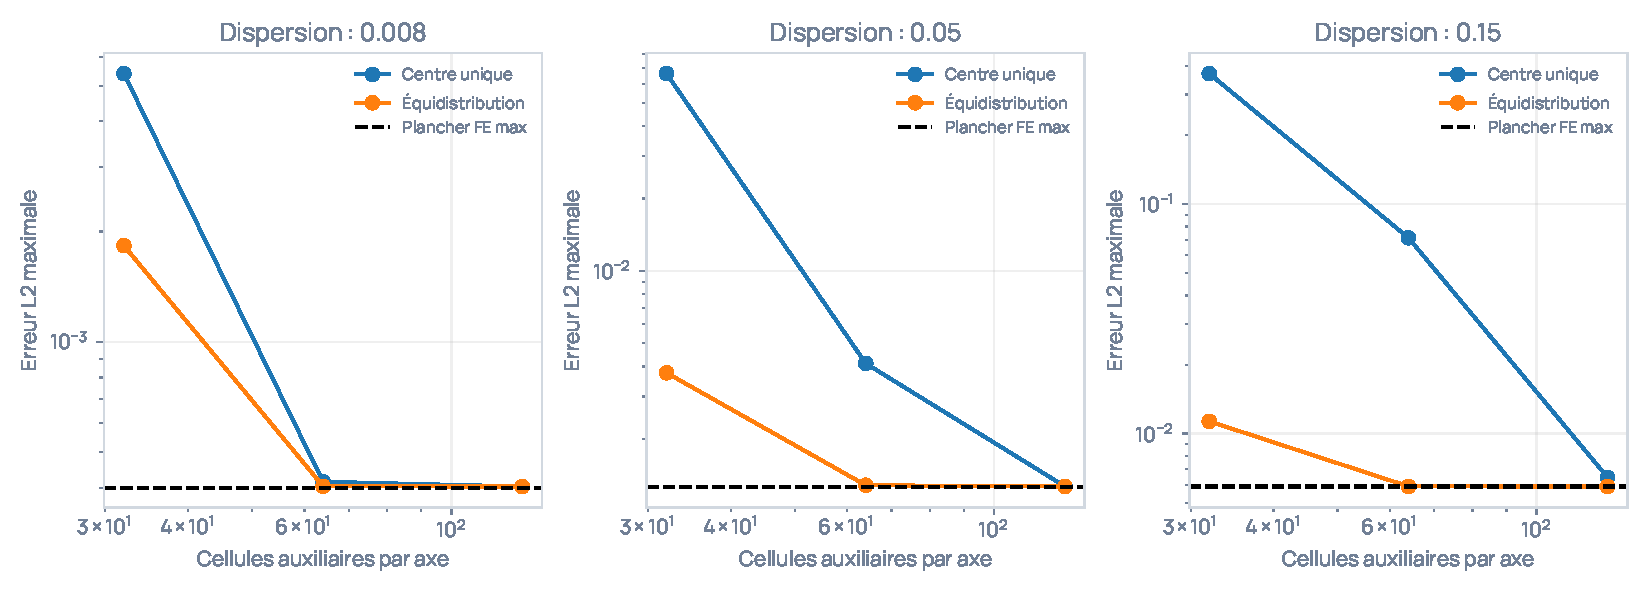
\includegraphics[width=.95\linewidth]{night-separated.pdf}\caption{Dix-huit cas à quatre champs et 128 pas. Le maillage FE est fixé : son plancher se dégrade lorsque des profils passent dans ses régions moins fines. Le moniteur d'énergie rapproche l'erreur de ce plancher, sans résoudre cette limite FE.}\end{figure}
\begin{figure}[htbp]\centering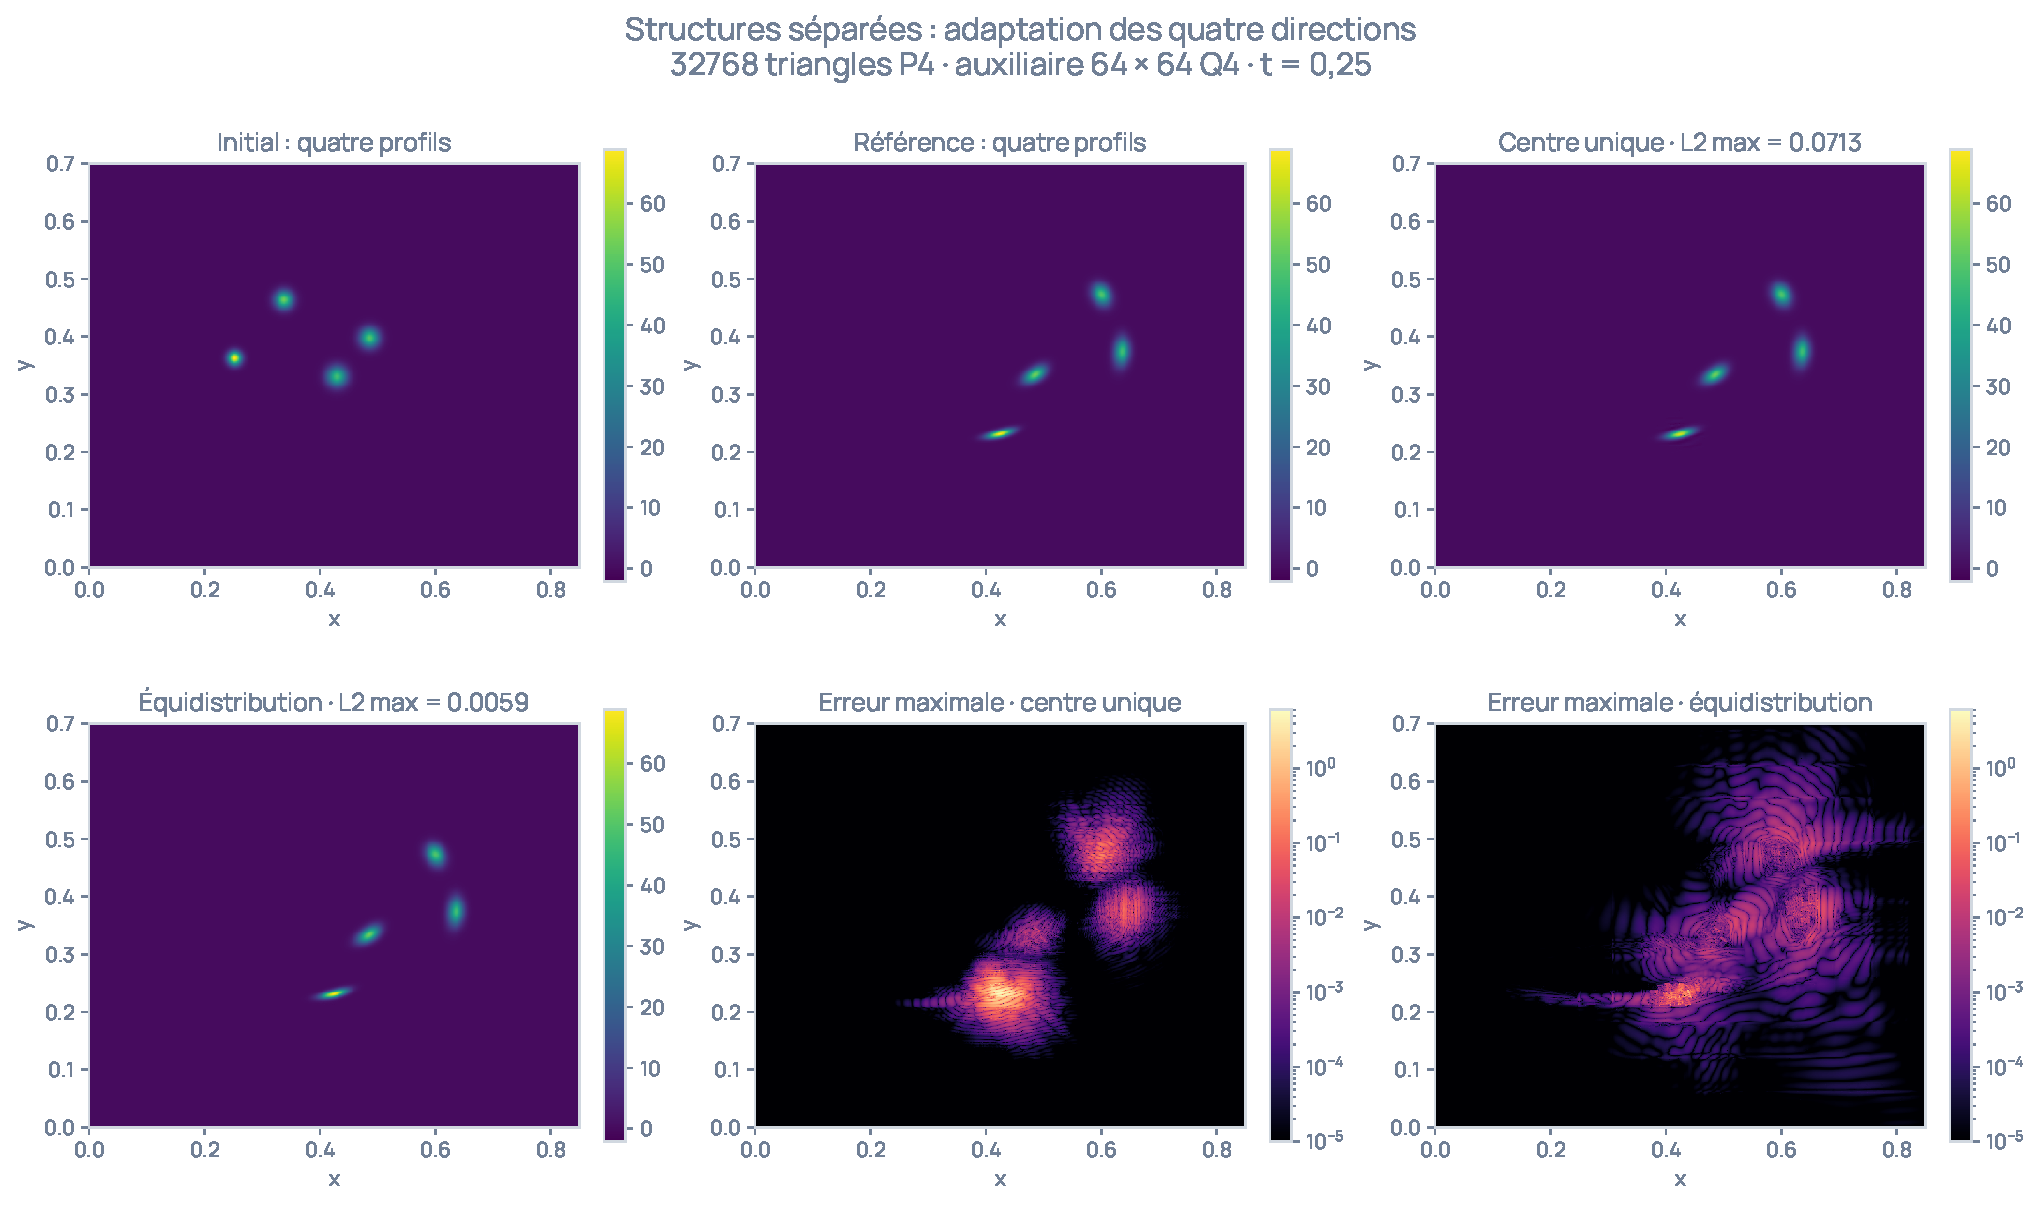
\includegraphics[width=.95\linewidth]{night-separated-fields.pdf}\caption{Champs calculés pour une dispersion 0,15. Les champs affichés sont les sommes des quatre profils; les cartes d'erreur prennent le maximum des erreurs ponctuelles individuelles. Les valeurs L2 indiquées sont les maxima sur les quatre champs.}\end{figure}
Extension au couplage FE : 12 cas disponibles avec quatre structures séparées, avec ou sans réaction. Le tableau inclut le maillage FE raffiné pour lever le précédent plancher. Les erreurs sont prises sur le pire des quatre champs.

\begin{center}\small\begin{tabular}{llllll}\toprule
FE n & Réaction & Support & Itér. & L2 max & Plancher max\\\midrule
128 & non & centre & 8 & 0.07137 & 0.005891\\
128 & non & énergie & 0 & 0.008536 & 0.005891\\
128 & non & énergie & 8 & 0.005928 & 0.005891\\
128 & oui & centre & 8 & 0.05704 & 0.004135\\
128 & oui & énergie & 0 & 0.005985 & 0.004135\\
128 & oui & énergie & 8 & 0.004161 & 0.004135\\
256 & non & centre & 8 & 0.0734 & 0.0003436\\
256 & non & énergie & 0 & 0.0009183 & 0.0003436\\
256 & non & énergie & 8 & 0.0009188 & 0.0003436\\
256 & oui & centre & 8 & 0.05817 & 0.0002408\\
256 & oui & énergie & 0 & 0.000704 & 0.0002408\\
256 & oui & énergie & 8 & 0.0007014 & 0.0002408\\
\bottomrule\end{tabular}\end{center}
Le raffinement FE révèle une erreur auxiliaire auparavant masquée. L'étude suivante augmente séparément le nombre de cellules auxiliaires et le nombre de pas, sur le maillage FE n=256. Une amélioration de mémoire ne peut pas supprimer une erreur d'advection ou de résolution dans le support auxiliaire.

\begin{center}\small\begin{tabular}{llllll}\toprule
Aux. n & Pas & Réaction & Itér. & L2 max & Plancher max\\\midrule
64 & 256 & non & 0 & 0.0005846 & 0.0003436\\
64 & 256 & non & 8 & 0.0005897 & 0.0003436\\
64 & 256 & oui & 0 & 0.0004556 & 0.0002408\\
64 & 256 & oui & 8 & 0.0004553 & 0.0002408\\
128 & 128 & non & 0 & 0.0004025 & 0.0003436\\
128 & 128 & non & 8 & 0.0003467 & 0.0003436\\
128 & 128 & oui & 0 & 0.0002809 & 0.0002408\\
128 & 128 & oui & 8 & 0.000243 & 0.0002408\\
128 & 256 & non & 0 & 0.0004471 & 0.0003436\\
128 & 256 & non & 8 & 0.0003447 & 0.0003436\\
128 & 256 & oui & 0 & 0.0003117 & 0.0002408\\
128 & 256 & oui & 8 & 0.0002416 & 0.0002408\\
\bottomrule\end{tabular}\end{center}
\section{Déformer puis revenir : erreur accumulée sans référence numérique}
Le flot autonome est suivi pendant une durée T, puis sa vitesse est inversée pendant la même durée. La solution exacte finale est le profil initial : aucune intégration de caractéristiques n'est nécessaire pour cette référence. Les partitions restent adaptées au champ calculé pendant les deux trajets. La dissipation et les pertes de mémoire ne s'annulent pas lors du retour.

\begin{center}\small\begin{tabular}{lllll}\toprule
Durée aller & Transfert & Changements & L2 max & Retour FE max\\\midrule
0.25 & reset & 63 & 0.006669 & 0.006668\\
0.25 & projected & 63 & 0.0008691 & 0.0008622\\
0.25 & chebyshev & 63 & 0.0007821 & 0.0007821\\
0.5 & reset & 63 & 0.06498 & 0.06498\\
0.5 & projected & 63 & 0.01545 & 0.01545\\
0.5 & chebyshev & 63 & 0.01491 & 0.01491\\
\bottomrule\end{tabular}\end{center}
Campagne de déformation élargie : 10 cas sur 48 enregistrés. Les erreurs affichées portent sur le pire des quatre champs; les cas qui n'atteignent pas la tolérance restent présents.

\begin{figure}[htbp]\centering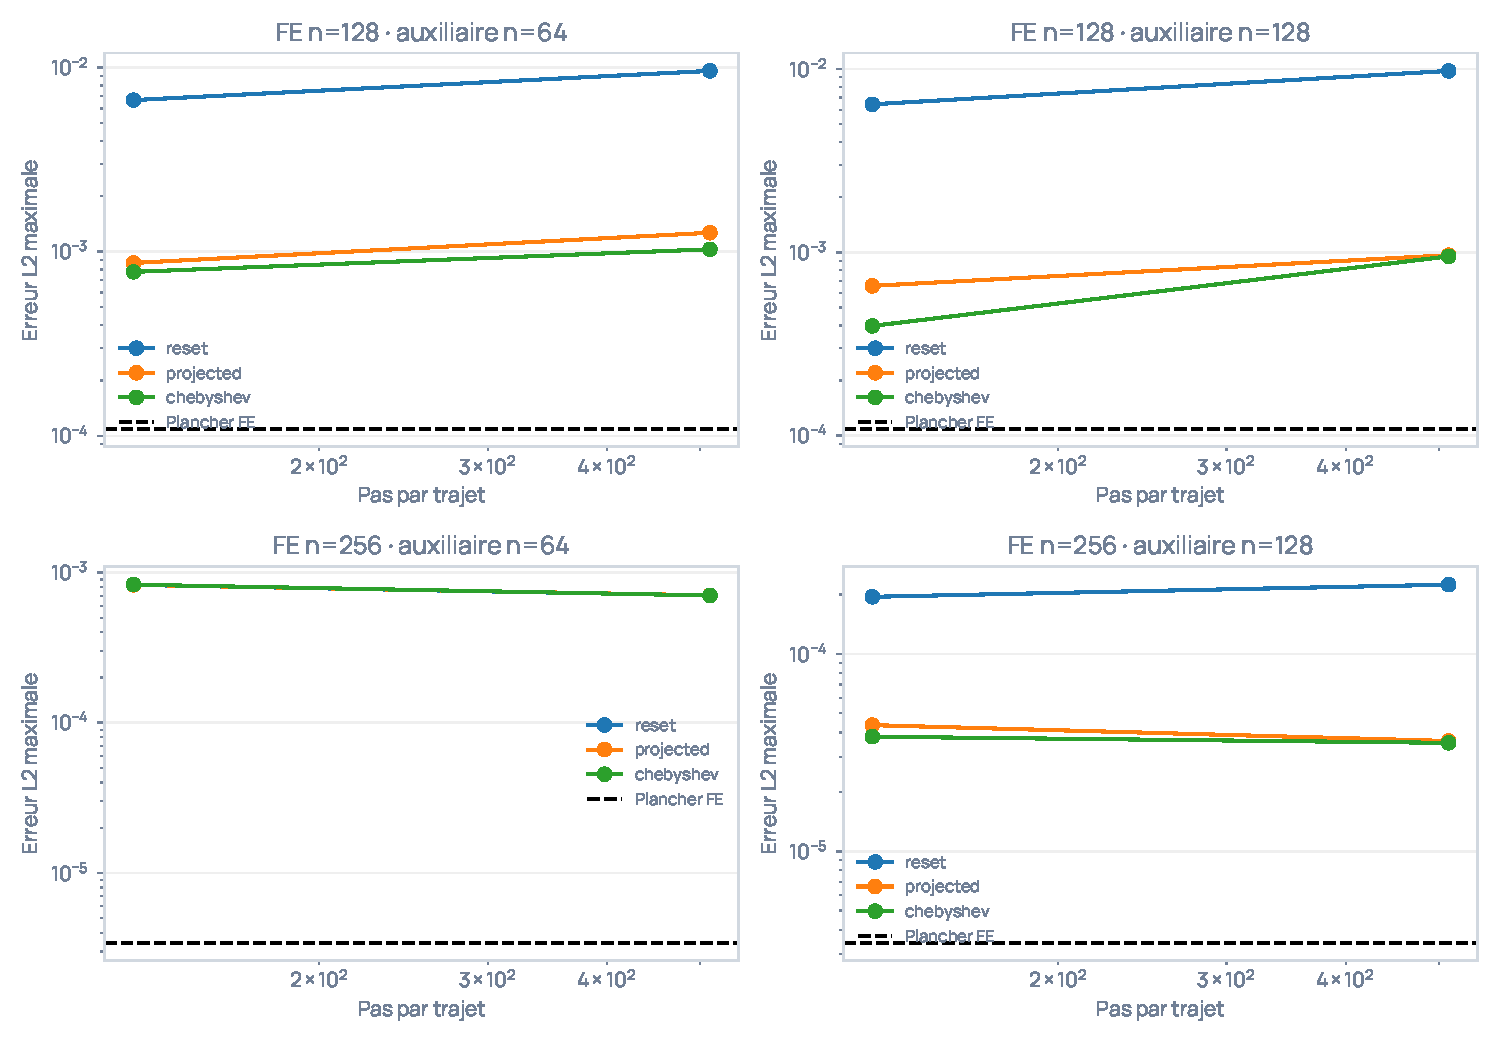
\includegraphics[width=.95\linewidth]{night-return-0-25.pdf}\caption{Aller-retour de durée totale 0.5. Le raffinement en temps et en espace est distingué. Un panneau vide signifie que le calcul correspondant n'est pas encore enregistré.}\end{figure}
\begin{figure}[htbp]\centering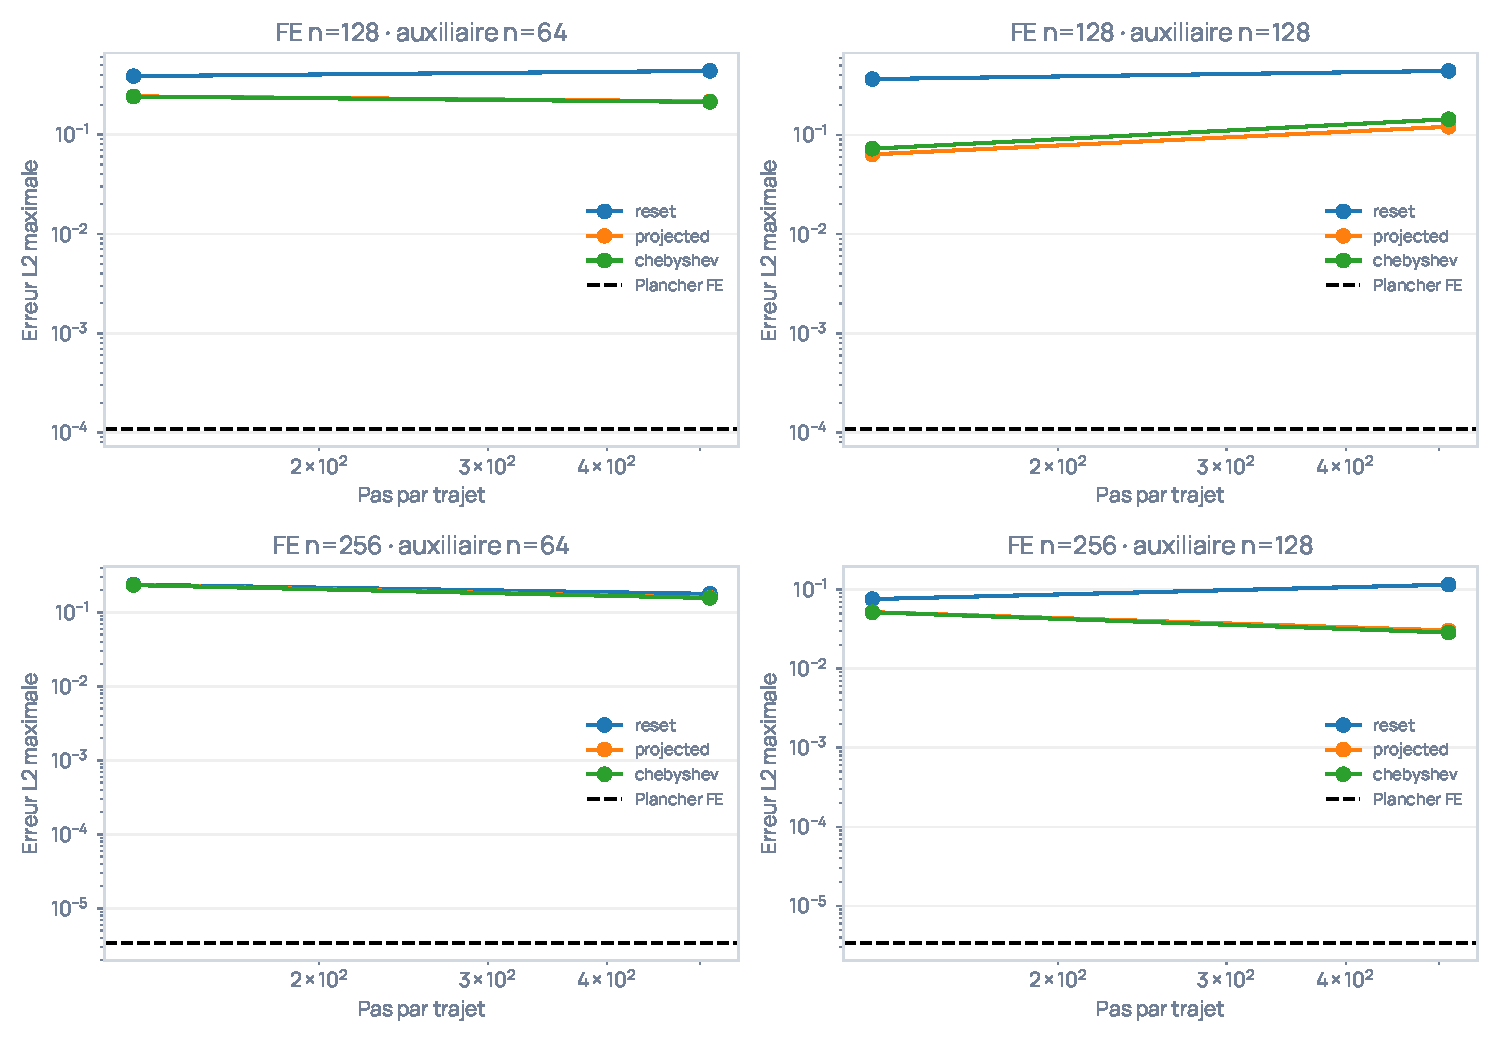
\includegraphics[width=.95\linewidth]{night-return-1-0.pdf}\caption{Aller-retour de durée totale 2.0. Le raffinement en temps et en espace est distingué. Un panneau vide signifie que le calcul correspondant n'est pas encore enregistré.}\end{figure}
\section{Exploration : vitesses issues de produits de fonctions de courant}
Une fonction de courant somme de produits a(y)b(x) transforme l'advection en somme de commutateurs de cisaillements. Le prototype réutilise une formule publiée de Casas, Escorihuela-Tomàs et Moreno Casares (2025), PCP16. Ses seize cisaillements Fourier sont unitaires; son ordre cinq dans la racine du pas correspond à l'ordre deux dans le temps physique, à grille fixée. Les coefficients et cette théorie de composition sont attribués aux auteurs. L'intérêt recherché ici est une extension des vitesses admissibles dans le couplage FE, dont la nouveauté et l'avantage de coût ne sont pas établis.

Les tests emploient un ou deux tourbillons gaussiens périodiques, dont la fonction de courant possède de nombreux modes de Fourier mais peu de produits séparables. Un oracle matriciel GPU contrôle le commutateur, l'unitarité, les constantes, l'inverse et le défaut temporel. Une intégration indépendante de caractéristiques contrôle l'erreur physique. Une erreur nodale RMS est distinguée de l'erreur FE intégrée.

\begin{figure}[htbp]\centering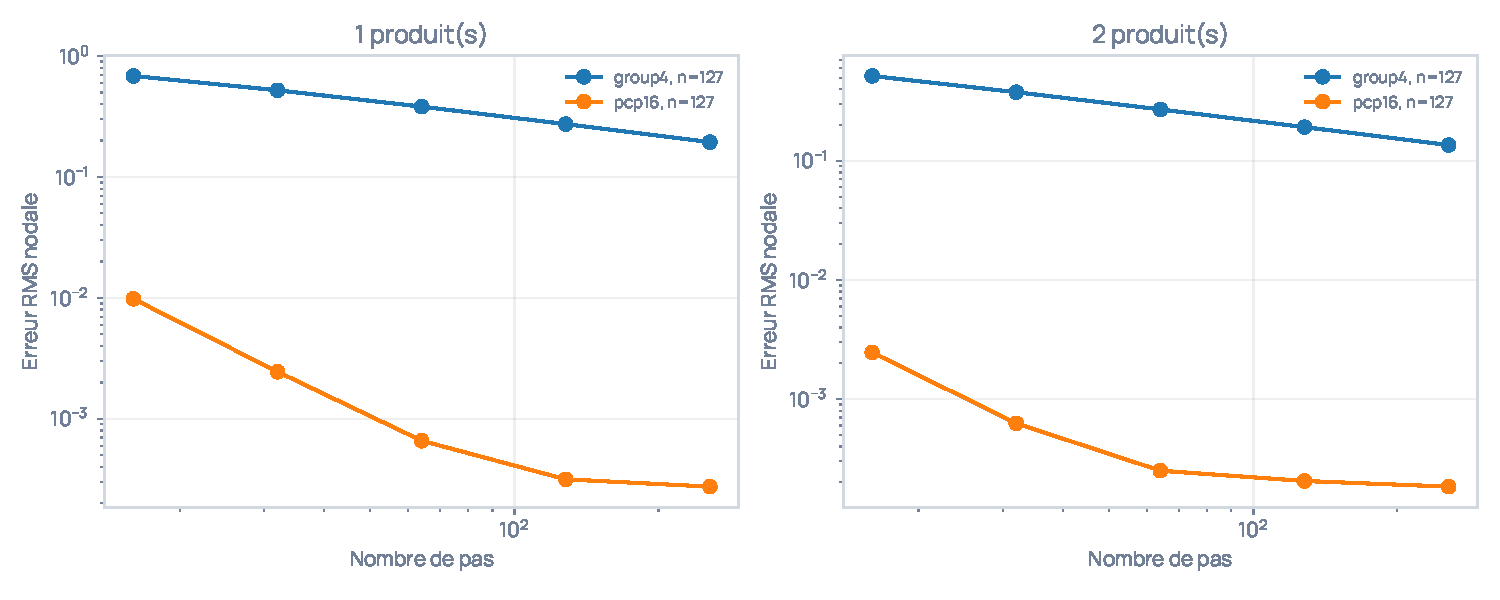
\includegraphics[width=.95\linewidth]{night-products.pdf}\caption{La grille de 127 points peut imposer un plancher spatial. Les résultats nodaux exploratoires ne constituent pas un benchmark de performance FE ni une validation d'une vitesse FE arbitraire.}\end{figure}
\section{Raffinement : identité validée, contrôleur insuffisant}
\begin{center}\small\begin{tabular}{llll}\toprule
Degré & Raffinement & Défaut Gram & Défaut observation\\\midrule
1 & global & 1.221e-15 & 6.661e-16\\
1 & local & 7.772e-16 & 5.551e-16\\
2 & global & 2.22e-15 & 1.11e-15\\
2 & local & 1.665e-15 & 1.221e-15\\
4 & global & 4.219e-15 & 3.386e-15\\
4 & local & 4.108e-15 & 3.209e-15\\
\bottomrule\end{tabular}\end{center}
Le premier contrôleur raffine selon la partie du générateur FE non représentée par le support. Les sélections par énergie et par détail hiérarchique atteignent toutes deux la limite de 96 intervalles dès le deuxième contrôle. L'erreur finale reste proche de 0,148. La conservation de l'énergie lors du raffinement ne répare donc pas ce contrôleur : le budget est épuisé tôt, et aucun déraffinement ne libère les cellules derrière la structure. L'indicateur utilisé ne mesure qu'un terme du défaut de consistance.

\begin{figure}[htbp]\centering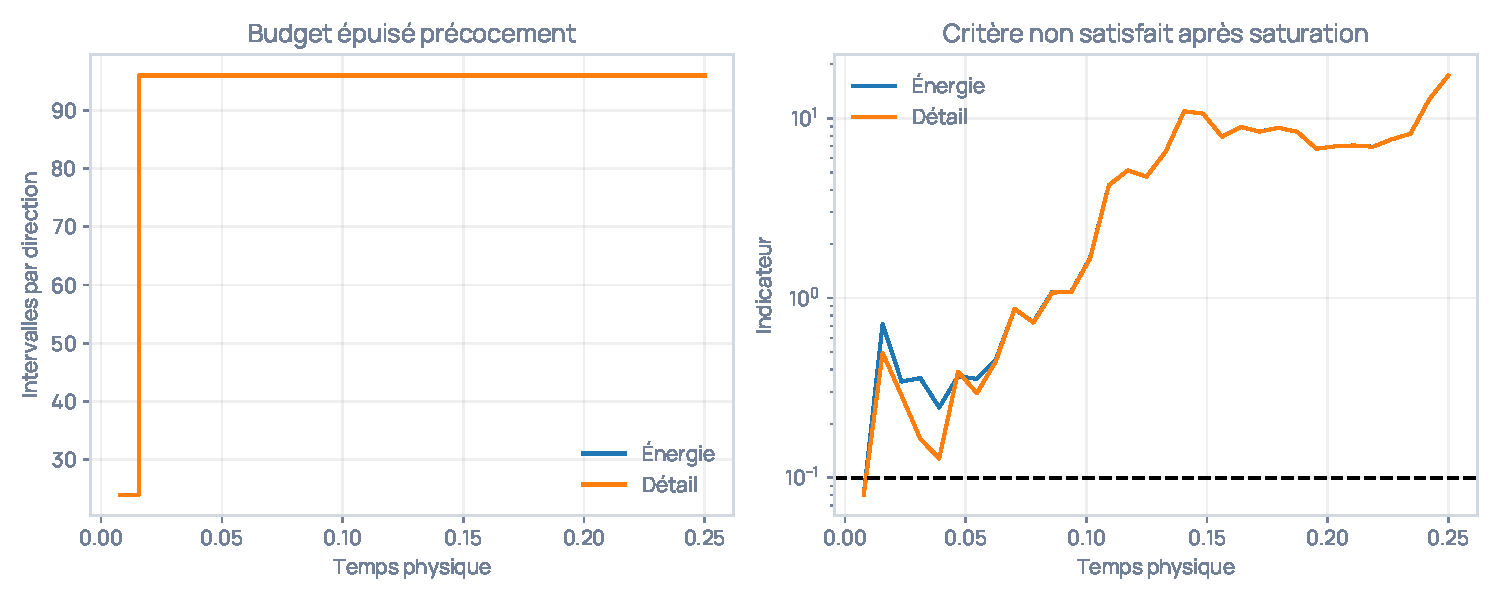
\includegraphics[width=.95\linewidth]{night-refinement.pdf}\caption{Résultat négatif conservé : changer le classement des cellules ne suffit pas à rendre le contrôleur efficace.}\end{figure}
\section{Contrôles et limites pour un article}
La note établit également une borne d'erreur pour des supports variables : une transition contractante qui envoie l'état minimal J\_n v sur J\_(n+1) v n'ajoute pas de terme explicite dépendant du nombre de remaillages. Les défauts locaux de transport restent dans la borne, notamment le commutateur entre projection et générateur. Ce résultat conditionnel ne fournit ni un ordre de convergence pour les noyaux actuels ni une garantie d'efficacité du contrôleur.

\begin{center}\small\begin{tabular}{lll}\toprule
Campagne & Enregistrés & Prévus\\\midrule
matched & 18 & 18\\
adaptive-physics & 24 & 24\\
adaptive-chebyshev & 12 & 12\\
moving-separated & 18 & 18\\
adaptive-separated & 12 & 12\\
memory-stress & 3 & 3\\
separated-refinement & 12 & 12\\
roundtrip-smoke & 6 & 6\\
roundtrip-long & 10 & 48\\
source-full & 0 & 16\\
products & 0 & 32\\
\bottomrule\end{tabular}\end{center}
nested-sanitizer : ========= ERROR SUMMARY: 0 errors

memory-transfer-sanitizer : ========= ERROR SUMMARY: 0 errors

ambient-sanitizer : ========= ERROR SUMMARY: 0 errors

chebyshev-sanitizer : ========= ERROR SUMMARY: 0 errors

energy-mesh-sanitizer : ========= ERROR SUMMARY: 0 errors

Les validations indépendantes couvrent les degrés 1, 2 et 4, les projections, les adjoints en masse, les constantes, les changements de support et les identités de Gram. Toutes les opérations numériques — recouvrements, quadrature, réductions, matrices denses de contrôle — sont exécutées sur CUDA. Le processeur pilote les expériences et dessine les figures. Il s'agit de prototypes isolés dans experiments/slfe, pas d'une intégration de production au langage variationnel Rodin.

La piste d'article est le couplage FE avec mémoire sur supports variables, accompagné de garanties d'énergie et de coût mesuré. Les conditions manquantes sont une erreur contrôlée pour des vitesses FE générales, un problème couplé où la mémoire apporte un bénéfice indispensable, un contrôleur robuste pour plusieurs structures et une comparaison avec des concurrents GPU plus proches. Le résultat actuel ne justifie pas une revendication de rupture.

\noindent\href{https://doi.org/10.1007/s11128-025-04659-z}{Casas, Escorihuela-Tomàs et Moreno Casares (2025), formules de commutateurs}\par
\noindent\href{https://arxiv.org/abs/2501.13681}{Adams, Finn, Knepley et Pusztay, rééchantillonnage par projection FE}\par
\noindent\href{https://gdz.sub.uni-goettingen.de/download/pdf/PPN362160546_0003/PPN362160546_0003.pdf}{Golub et Varga (1961), semi-itérations de Chebyshev}\par
\noindent\href{https://www.oca.eu/images/LAGRANGE/pages_perso/nbesse/pub/NBesse_jcp17.pdf}{Besse, Deriaz et Madaule (2017), adaptation multirésolution SL-DG}\par
\noindent\href{https://arxiv.org/abs/2603.19959}{Adams (2026), recouvrements SL-DG sur grilles adaptatives}\par
\noindent\href{https://cseweb.ucsd.edu/~ravir/sinasiga.pdf}{Nabizadeh et al. (2024), CO-FLIP et remise à zéro des cartes de flot}\par
\noindent\href{https://arxiv.org/abs/2212.03036}{Einkemmer et Moriggl, SL-DG sur GPU}\par
\section{Reproduction}
Les sources sont dans experiments/slfe : matched\_benchmark.py, adaptive\_study.py, moving\_study.py, refinement\_study.py, nested\_validation.py et ambient\_validation.py. Les fichiers results\_night2 contiennent les paramètres, erreurs, historiques et empreintes du code. night\_fields.py reproduit les champs; night\_report.py reconstruit ce rapport sans simulation; restart\_theory.tex fournit les hypothèses et preuves. Publication exclusivement sur la branche SLFE du fork keckj/rodin.
\end{document}